% !TeX program = pdflatex

\documentclass[12pt,a4paper,oneside,onecolumn]{book}

\usepackage[margin=2cm]{geometry}
\usepackage{libertine}
\usepackage{courier}
\usepackage[utf8x]{inputenc}
\usepackage[english]{babel}
\usepackage[longnamesfirst,square,numbers,comma,sort&compress]{natbib}
\usepackage{titlesec}
\usepackage{float}
\usepackage{graphicx}
\usepackage{amsmath}
\usepackage{mathpazo}
\usepackage{datetime}
\usepackage{mdframed}
%\usepackage{hyperref}
%\usepackage{bookmark}

\numberwithin{equation}{subsection}

\setcounter{secnumdepth}{3} % Include numbering for \subsubsection (and below)
\setcounter{tocdepth}{3}    % Include \subsubsection in the table of contents


\setlength{\parindent}{0pt}
\setlength{\parskip}{5pt}

\titleformat{\chapter}[hang]{\bf\huge}{\thechapter}{2pc}{}
\title{HUJI M.Sc.~Thesis Template}

\begin{document}

\begin{titlepage}
    \begin{center}
        \vspace*{1cm}
        
        
\includegraphics[width=0.15\textwidth]{images/huji_logo_notext.pdf}\\
        The Hebrew University of Jerusalem\\
        The Rachel and Selim Benin School of Computer Science and Engineering
        
        \vspace{2cm}
        
        {\Large \textbf{TEMPOTRON WITH GLOBAL GATING }}
        
        % \vspace{1cm}
        % {\Large secondary title}
        % \vspace{1.5cm}
        
        \textbf{Roy Michaeli and Haim Sompolinsky}
        
        \vspace{1cm}
        
        Thesis submitted in partial fulfillment of the requirements\\for the Master of Sciences degree\\
        in Computer Science
        
        \vspace{1cm}
        
        Under the supervision of \textbf{Prof Haim Sompolinsky}
        
        \vfill
        
        \textbf{Month year}
    \end{center}
\end{titlepage}
%\begin{titlepage}
    \begin{center}
        \vspace*{1cm}
        
        
\includegraphics[width=0.5\textwidth]{huji_logo_hor.pdf}\\
        The Hebrew University of Jerusalem\\
        The Rachel and Selim Benin School of computer Science and Engineering
        
        \vspace{2cm}
        
        {\Large \textbf{Thesis Title}}
        
        \vspace{1.5cm}
        
        \textbf{Author}
        
        \vspace{1cm}
        
        Thesis submitted in partial fulfillment of the requirements\\for the Master of Sciences degree
        
        \vspace{1cm}
        
        Under the supervision of \textbf{Supervisor}
        
        \vspace{1cm}
        
        \begin{flushleft}
        Signature of student: \( \rule{3cm}{0.15mm} \) \hfill Date: \( \rule{3cm}{0.15mm} \)\\
        Signature of supervisor: \( \rule{3cm}{0.15mm} \) \hfill Date: \( \rule{3cm}{0.15mm} \)\\
        Signature of chairperson of the\\committee for graduate studies: \( \rule{3cm}{0.15mm} \) \hfill Date: \( \rule{3cm}{0.15mm} \)
        \end{flushleft}
        
        \vfill
        
        \textbf{Month Year}
    \end{center}
\end{titlepage}

\frontmatter

\renewcommand{\baselinestretch}{1.5}

\chapter*{Abstract}

this is where the future abstract will be.
\chapter*{Acknowledgements}

Do I really want to thank anyone?

\tableofcontents
\listoffigures
\listoftables

\mainmatter 

\chapter{Introduction}
\label{chap:intro}

The Tempotron model \cite{gutig2006tempotron}, introduced by Gütig and Sompolinsky in 2006, is a neural network model that focuses on temporal coding and processing of information in spiking neural networks. It builds upon previous research in computational neuroscience and aims to capture the temporal dynamics of neural networks, specifically in the context of pattern recognition tasks. The Tempotron model has garnered attention and been extensively studied in the field, including its application on datasets such as the MNIST dataset, which is widely used for benchmarking machine learning algorithms.
\chapter{Scientific Background}

\label{chap:sb}

\section{Artificial Neural Networks}

The Perceptron model served as a fundamental building block for numerous advancements and paved the way for developing more sophisticated techniques. Some key developments that have significantly enhanced the capabilities of neural networks include:

\subsection{Back-propagation}

To extend the perceptron model's learning capabilities, the concept of backpropagation was introduced. This algorithm, initially proposed by Paul Werbos in 1974, revolutionized neural network training by efficiently propagating error gradients backward through the layers of the network. By iteratively adjusting the weights based on these gradients, backpropagation enabled neural networks to learn complex patterns and improve their performance.

\subsection{Activation functions}

The perceptron model originally employed a single layer with a threshold activation function, which limited its ability to handle non-linearly separable problems. However, the introduction of various activation functions over the years, such as the Rectified Linear Unit (ReLU), parametric ReLU, hyperbolic tangent (tanh), and sigmoid functions, played a crucial role in neural networks by introducing non-linearities to the output of each neuron. The concept of activation functions in neural networks traces back to the early foundation of the field. While there have been numerous contributions and refinements, the incorporation of activation functions can be attributed to Warren McCullen and Walter Pits in the 1940s \cite{mcculloch1943logical}. They introduced the Heaviside activation function, which later inspired the development of ReLU and its variants.
By using activation functions, neural networks gained the ability to model complex and nonlinear relationships. This allowed the construction of deeper architectures with multiple layers, enabling networks to learn hierarchical representations and capture intricate features in the input data.
These advancements in backpropagation and activation functions have played a crucial role in the development of neural networks. They have enabled the training of deeper, more complex architectures and facilitated the modeling of non-linear relationships, making neural networks more powerful and versatile in solving various problems.


\subsection{Cost Function}

Loss or cost function, also known as the objective function, is a fundamental component in the training process of neural networks. It quantifies the discrepancy or error between the predicted outputs of the network and the true target values, serving as a measure of how well the network is performing.
The cost function plays a crucial role in training by providing a quantitative measure of the network's performance, enabling the optimization algorithms to adjust the network's parameters, typically the weights, to minimize the cost. One commonly used optimization algorithm is gradient descent, which relies on the differentiability of the cost function to compute the gradients and update the weights iteratively. The network aims to reduce the prediction error and improve its performance on unseen data by minimizing the cost function over the training data.
However, it is important to note that not all cost functions are differentiable. In certain cases, non-differentiable cost functions may be encountered, which poses challenges for optimization algorithms that rely on gradient-based methods. Non-differentiability can occur when the cost function involves non-smooth operations, such as max or absolute value functions. In such situations, alternative optimization techniques, such as subgradient methods or heuristics, may be employed to approximate the optimal solution.
Over the years, various objective functions have been proposed and studied, each with its own characteristics and suitability for different tasks. For classification tasks, common choices of cost functions include cross-entropy, Mean Squared Error (MSE), and Mean Absolute Error (MAE). These functions have shown promising results and have been extensively used in neural network research.


\subsection{Optimizers}

Optimizers play a crucial role in effectively training neural network models, and numerous approaches and algorithms have been proposed in recent years. Among the approaches employed in our work, Stochastic Gradient Descent (SGD) is the primary optimization technique utilized. This approach involves the partitioning of the training data into smaller randomly selected subsets. By iterating over these subsets, the model's parameters are updated with respect to the examples within each subset, facilitating the learning process.
Algorithmic optimizers, on the other hand, represent another category of optimizers that dynamically compute the learning rate based on current and past gradients. Some well-known optimizers in this category include Momentum, AdaGrad, and ADAM. These optimizers have gained recognition for their ability to enhance training efficiency and convergence in neural network models.


\section{Computational Models}

The field of computational neuron models seeks to comprehend and simulate the behavior of individual neurons in the brain using mathematical and computational methods. Over time, neuron models have evolved from simplistic abstractions to more intricate and biologically realistic representations. In 1907, Lapicque \cite{abbott1999lapicque} conducted significant research on the impact of current source stimuli on the nerve fiber of a frog's leg [4]. Through his investigation, he observed the influence of stimuli amplitude and duration on the leg's twitching response. He proposed that a spiking neuron can be analogously modeled as a low-pass filter circuit, consisting of a capacitor (C) and a resistor (R). This concept was later referred to as the Leaky Integrated and Fire (LIF) neuron.
Various spiking neuron models exist alongside the Leaky Integrate-and-Fire (LIF) neuron. Some notable models are described below:

\begin{itemize}

    \item The Leaky Integrate-and-Fire model (LIF): Represents the dynamics of a neuron's membrane potential. It models the neuron's behavior by integrating incoming current over time and then "fires" (produces an action potential) when the potential reaches a certain threshold. The equation is given by:
    
    \begin{equation}
    \tau_m \frac{{dV}}{{dt}} = -(V(t) - V_{\text{rest}}) + R \cdot I(t)
    \end{equation}
    
    where:
    \( \tau_m \) is the membrane time constant,
    \( V \) is the membrane potential,
    \( V_{\text{rest}} \) is the resting membrane potential,
    \( R \) is the membrane resistance,
    and \( I(t) \) is the input current.
    
    The leak factor, often denoted as \( \beta \), determines the strength of the leak current in the neuron. It is related to the membrane resistance \( R \) as \( \beta = \frac{1}{R} \).

    \item Integrate-and-Fire (IF): This model removes the leakage mechanism, resulting in β = 1 in Equation (?)  #TODO: add equation.
    
    \item Current-based (CuBa): Commonly referred to as CuBa neuron models, these incorporate synaptic conductance variation into leaky integrate-and-fire neurons. Unlike the default LIF neuron, CuBa neurons act as second-order low-pass filters, introducing a finite rise time for the membrane potential rather than abrupt jumps in response to incoming spikes [add citation]. Figure (?) illustrates a depiction of a neuron with a finite rise time for the membrane potential.
    
    \item Recurrent Neurons: In this model, the output spikes of a neuron are fed back to the input, as indicated by explicit recurrence in Figure (?). Recurrence is not an alternative model but rather a topology that can be applied to any neuron. It can be implemented in different ways, such as one-to-one recurrence, where each neuron routes its own spike back to itself, or all-to-all recurrence, where the output spikes of a full layer are weighted and summed before being fed back to the entire layer [?] #TODO: add citation!.

    \item Kernel-based Models: Also known as spike-response models, these models convolve input spikes with a predefined kernel, such as the 'alpha function' [?] #TODO: add citation. The ability to define the kernel shape provides significant flexibility.

    \item Deep learning-inspired spiking neurons: Instead of drawing inspiration solely from neuroscience, these models incorporate concepts from deep learning by applying spiking thresholds. This approach extends the short-term capacity of basic recurrent neurons. Examples include spiking LSTMs [?] #TODO: add citation! and Legendre Memory Units [?] #TODO: add citation!. Recent advancements involve the utilization of transformers to enhance long-range memory dependencies in data. SpikeGPT approximated self-attention into a recurrent model, demonstrating natural language generation with SNNs for the first time [?] #TODO: add citation!.

    \item Higher-complexity neuroscience-inspired models: A wide range of more detailed neuron models exist, incorporating biophysical realism and/or morphological details that are not captured by simple leaky integrators. Well-known models in this category include the Hodgkin-Huxley model [?] and the Izhikevich (or Resonator) model [?], which offer improved accuracy in reproducing electrophysiological results.
    
\end{itemize}

These diverse spiking neuron models cater to different research interests, incorporating varying levels of biological realism, morphological complexity, and applicability to specific tasks within the field of neural computing.


\section{The Tempotron}

The Tempotron model is a computational neural network specifically designed for spike-time-based pattern recognition. Training the Tempotron involves optimizing the synaptic weights to achieve accurate pattern recognition based on the timing of input spikes. Different researchers have proposed several methods over the years to train the Tempotron model effectively. Here is an overview of some notable methods and the researchers associated with their development:
\begin{itemize}

    \item Tempotron Training Algorithm: In 2006, Gütig and Sompolinsky \cite{gutig2006tempotron} introduced a training algorithm for the Tempotron model based on spike-time-dependent plasticity (STDP). Their work focused on adjusting the synaptic weights using a reinforcement learning approach, where potentiation and depression of synapses were governed by the timing of pre and post-synaptic spikes. This algorithm enabled the Tempotron to learn to recognize spatiotemporal patterns.
    
    \item 	Supervised Tempotron Learning: Bohte, Kok, and La Poutré \cite{bohte2002error} proposed a supervised learning approach for training the Tempotron in 2002. Their method used gradient descent optimization to adjust the synaptic weights based on the error between the target output and the actual output of the Tempotron. The Tempotron was trained to improve its accuracy in recognizing spike-time patterns by iteratively updating the weights.
    
    \item Reinforcement Learning for Tempotron: In 2011, Ponulak and Kasiński \cite{ponulak2011introduction} presented a reinforcement learning algorithm to train the Tempotron model. Their approach utilized a reward-based mechanism, where the Tempotron received positive or negative reinforcement signals based on its classification performance. By maximizing the cumulative reward signal, the Tempotron adapted its synaptic weights to enhance pattern recognition capabilities.
    
    \item SpikeProp Algorithm: Bohte, Kok, and La Poutré \cite{bohte2002error} also developed the SpikeProp algorithm in 2000, which was specifically designed to train networks of spiking neurons, including the Tempotron model. SpikeProp utilized error backpropagation principles but adapted them to account for the discrete nature of spikes. This algorithm enabled efficient weight updates in the Tempotron based on the discrepancy between the target spike train and the generated output spikes.
    
    \item Unsupervised Tempotron Learning: Masquelier and Thorpe \cite{masquelier2007unsupervised} introduced an unsupervised learning algorithm for the Tempotron in 2007. Their method focused on training the Tempotron using Hebbian learning, which modifies the synaptic weights based on correlated activity between pre- and post-synaptic neurons. This unsupervised approach allowed the Tempotron to learn to recognize complex temporal patterns without explicit target labels.

These are just a few examples of the various methods proposed to train the Tempotron model. Each method brings its own insights and techniques to improve the learning capabilities of the Tempotron. Researchers have continued to refine and extend these methods over time, contributing to the advancement of spike-based pattern recognition and the broader field of spiking neural networks.

\end{itemize}




\chapter{Motivation}
\label{chap:motivation}


\chapter{Previous Work}
\label{chap:pw}


\chapter{Research Question}
\label{chap:rq}

\section*{Research Question 1}
\textit{How can gating mechanisms be integrated into the Tempotron model to enhance the training efficiency and performance of Spiking Neural Networks?}

\textbf{Elaboration:}
This research question aims to investigate the integration of gating mechanisms, Gating Units, and different cost functions into the Tempotron model for training Spiking Neural Networks (SNNs). The study will explore how the inclusion of gating mechanisms can enhance the network's ability to capture temporal patterns and context in spiking patterns. The research will involve the design and implementation of novel variations of the Tempotron model that incorporate gating mechanisms. Training efficiency and performance metrics, such as classification accuracy, sparsity, and computational resources, will be compared between the original Tempotron model and the modified versions with gating. The investigation will also focus on understanding the impact of gating mechanisms on training stability and generalization in SNNs.

\section*{Research Question 2}
\textit{What are the most effective backpropagation techniques that can be adapted and applied to the Tempotron model for training Spiking Neural Networks, and how do they compare in terms of convergence speed and accuracy?}

\textbf{Elaboration:}
This research question aims to explore various backpropagation techniques adapted for training SNNs using the Tempotron model. The study will evaluate the convergence speed and accuracy achieved by each backpropagation variant during the training process. Comparisons will be made based on their performance across different datasets and SNN architectures. Additionally, the research will delve into the computational requirements and memory usage of each backpropagation technique to assess their suitability for real-time and energy-efficient applications in SNNs.

\section*{Research Question 3}
\textit{What strategies can be employed to overcome the computational challenges of training large-scale Spiking Neural Networks in the context of the Tempotron model, and how do these strategies impact the network's performance and resource requirements?}

\textbf{Elaboration:}
The performance and resource requirements of SNNs trained with these strategies will be compared with conventionally trained networks. The research will also explore how these approaches impact the network's accuracy and sparsity. Additionally, considerations will be given to the scalability of these strategies for even larger SNN architectures, paving the way for more practical and resource-efficient implementations.



\chapter{Methods}
\label{chap:methods}

\subsection{Leaky Integrated and Fire Neuron}

\label{ch:computational-models}

\subsubsection{Introduction}

First, we will look at the basic equation from which we will learn about the behavior of the neuron according to this model:

\begin{equation}
v(t) + \tau_m \cdot \frac{dv(t)}{dt} = E_{\text{rest}} + R_m \cdot I_{\text{input}}
\end{equation}

If we set \( R_m = 1 \) and \( E_{\text{rest}} = 0 \), the equation becomes:

\begin{equation}
v(t) + \tau_m \cdot \frac{dv(t)}{dt} = I_{\text{input}}
\end{equation}

This is a first-degree differential equation with the conditions:

\begin{equation}
v(t=0) = v_{\text{reset}}
\end{equation}

\begin{equation}
v(t=\infty) = I_0
\end{equation}

We will "guess" a solution: 

\begin{equation}
v(t) = A \cdot \exp(\alpha \cdot t) + B
\end{equation}

Our initial equation will be:

\begin{equation}
t=0 : \quad A + B = v_{\text{reset}}
\end{equation}

\begin{equation}
t=\infty : \quad B = I_0
\end{equation}

So, \( A = v_{\text{reset}} - I_0 \) and \( B = I_0 \). Substituting these values, we get:

\begin{equation}
v(t=0) + \tau_m \cdot \frac{dv(t=0)}{dt} = A + B + \tau_m \cdot A \cdot \alpha = I_0
\end{equation}

\begin{equation}
v_{\text{reset}} + \tau_m \cdot (v_{\text{reset}} - I_0) \cdot \alpha = I_0
\end{equation}

Subtracting \( v_{\text{reset}} \) from each side and dividing by \( (v_{\text{reset}} - I_0) \) to get:

\begin{equation}
\alpha = -\frac{1}{\tau_m}
\end{equation}

Overall, our solution will be:

\begin{equation} \label{eq:general_sol}
v(t) = (v_{\text{reset}} - I_0) \cdot \exp(-t/\tau_m) + I_0
\end{equation}

Now we wish to see how long it takes for our neuron to reach action potential after the most recent spike:

After \( \Delta t = t_{\text{ref}} \) the neuron will start "charging" once more (refractory period). Our initial values are as we described – we want to find a value \( t \) which will give the following:

\begin{equation}
v(t) = v_{\text{thr}}
\end{equation}

This equation has two different states – if \( I_0 < v_{\text{thr}} \) the equation has no solutions! If \( I_0 \geq v_{\text{thr}} \):

\begin{equation}
(v_{\text{reset}} - I_0) \cdot \exp(-t/\tau_m) + I_0 = v_{\text{thr}}
\end{equation}

\begin{equation}
\exp(-t/\tau_m) = \frac{v_{\text{thr}} - I_0}{v_{\text{reset}} - I_0}
\end{equation}

\begin{equation}
t = \tau_m \cdot \ln\left(\frac{v_{\text{reset}} - I_0}{v_{\text{thr}} - I_0}\right)
\end{equation}

Since our input is constant, the behavior we just got will repeat itself after each firing – in other words; the neuron will fire after:

\begin{equation}
T = t_{\text{ref}} + \tau_m \cdot \ln\left(\frac{v_{\text{reset}} - I_0}{v_{\text{thr}} - I_0}\right)
\end{equation}

So, the firing frequency is given by:

\begin{equation}
f(I_E) = \begin{cases}
    0, & \text{if } I_E < v_{\text{thresh}} \\
    \left(t_{\text{ref}} + \tau_m \cdot \ln\left(\frac{I_E - V_{\text{reset}}}{I_E - V_{\text{thresh}}}\right)\right)^{-1}, & \text{else}
\end{cases}
\end{equation}

In conclusion, we reached the frequency function:

\begin{equation}
f(I_E) = \begin{cases}
    0, & \text{if } I_E < v_{\text{thresh}} \\
    \left(t_{\text{ref}} + \tau_m \cdot \ln\left(\frac{I_E - V_{\text{reset}}}{I_E - V_{\text{thresh}}}\right)\right)^{-1}, & \text{else}
\end{cases}
\end{equation}

Now we will look at some graphs that express the influence of the \( t_{\text{refractory}} \) and \( I_E \) values on the firing frequency.

\begin{figure}[H]
    \centering
    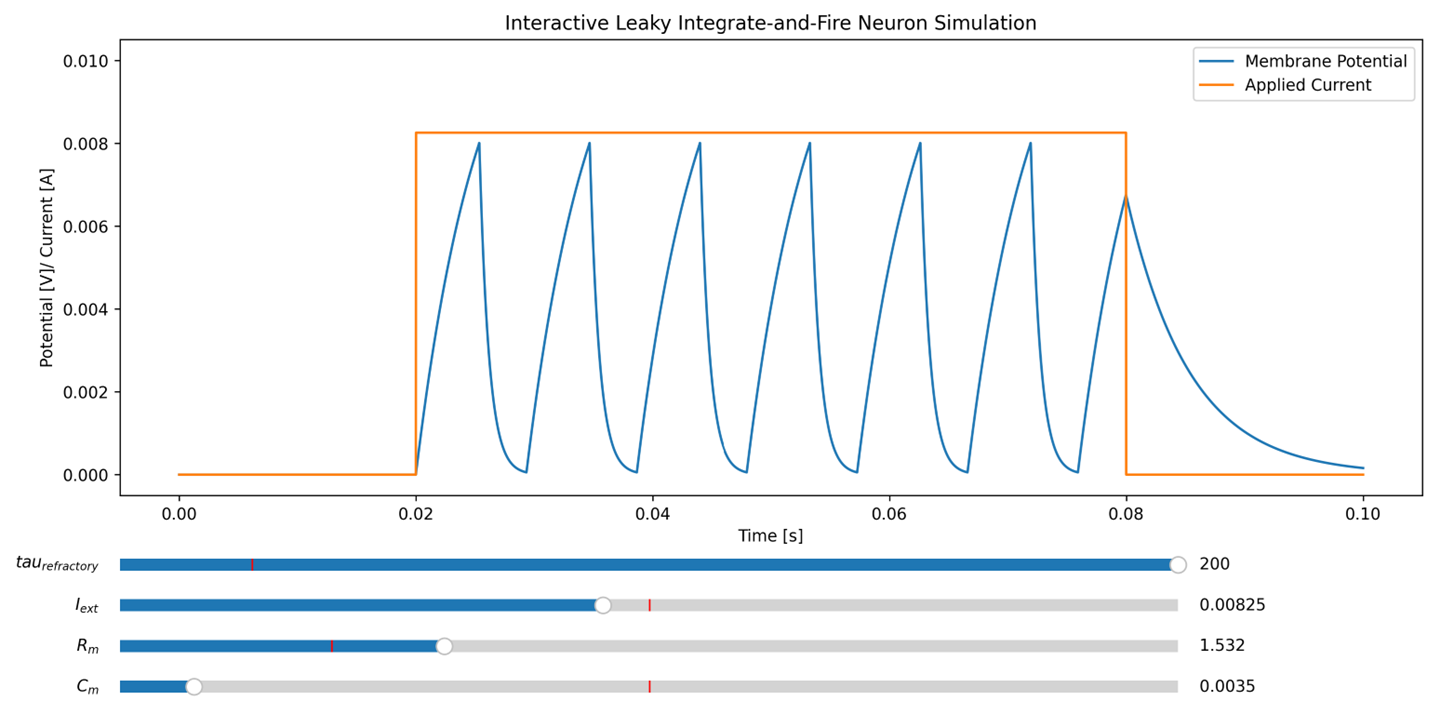
\includegraphics[width=0.8\textwidth]{methods/computational-models/graphs/LIF-heaviside-high-ref.png}
    \caption{High applied current with high refractory period gives low frequency}
    \label{fig:LIF-heaviside-high-ref}
\end{figure}

\begin{figure}[H]
    \centering
    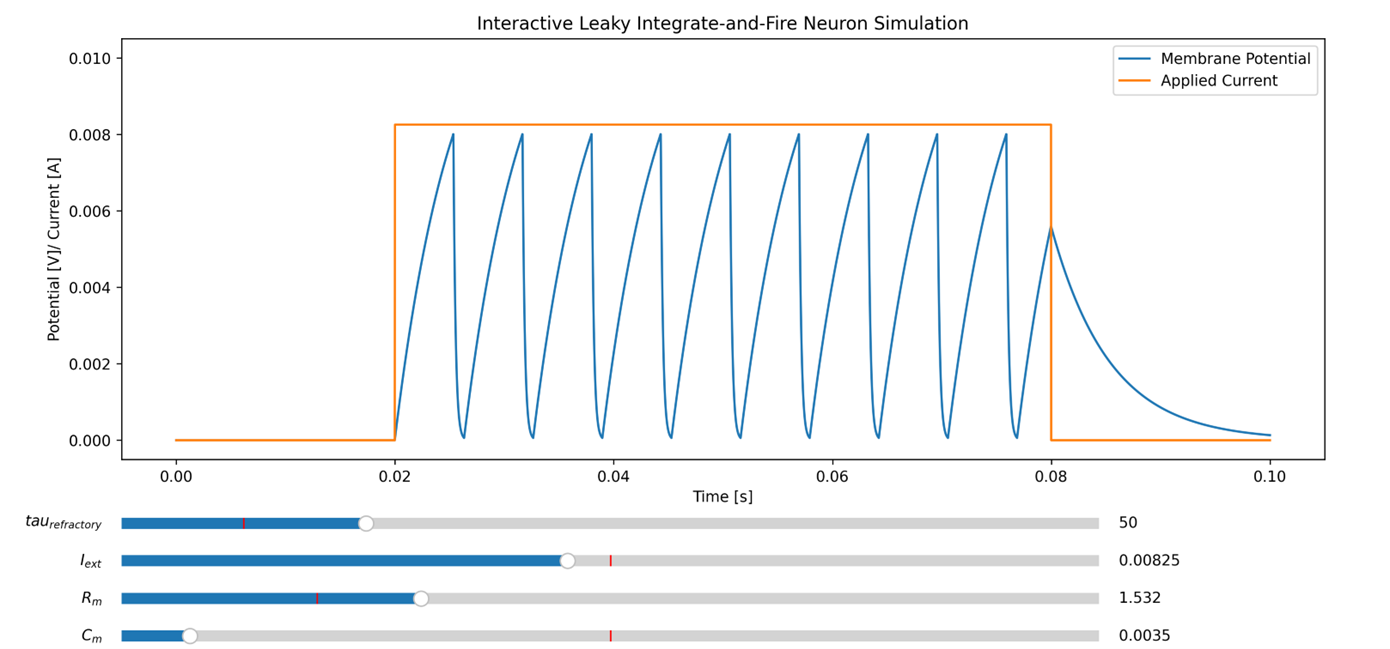
\includegraphics[width=0.8\textwidth]{methods/computational-models/graphs/LIF-heaviside-low-ref.png}
    \caption{High applied current with low refractory period gives higher frequency}
    \label{fig:LIF-heaviside-low-ref}
\end{figure}

\begin{figure}[H]
    \centering
    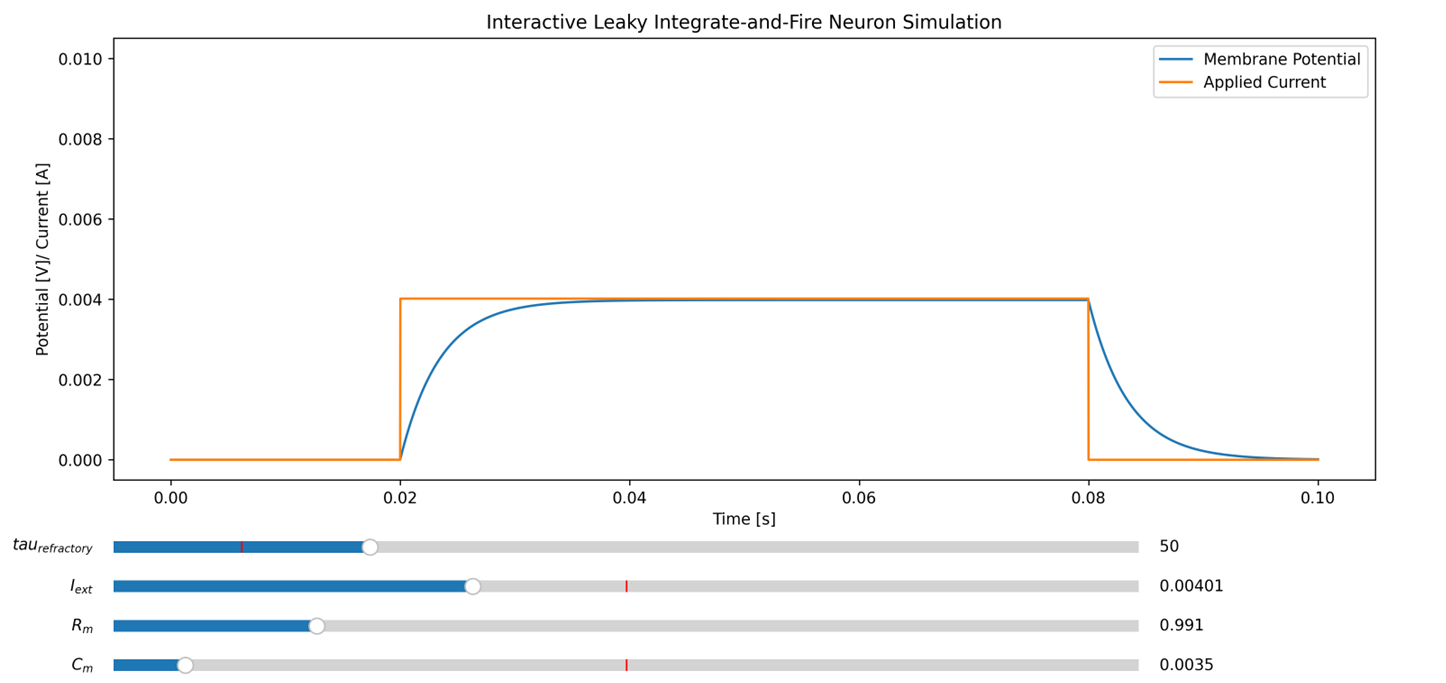
\includegraphics[width=0.8\textwidth]{methods/computational-models/graphs/LIF-heaviside-low-input.png}
    \caption{Low applied current will prevent the neuron from firing}
    \label{fig:LIF-heaviside-low-input}
\end{figure}

The refractory period is a period after firing of a specific neuron during which it will ``ignore'' the input current. We can demonstrate that behavior by the following equation:
*For this example, we assume that the neuron fired at \( t=0 \).
\begin{equation}
\forall t \in (0,\tau_{\text{ref}}), \quad I(t) = v_{\text{reset}}
\end{equation}
\begin{equation}
v(t=0) = v_{\text{thresh}}
\end{equation}
\begin{equation}
v(t) + \tau_m \cdot \dot{v}(t) = v_{\text{reset}}
\end{equation}
We already solved a similar equation \ref{eq:general_sol}, so the following solution will be:
\begin{equation}
v(t) = (v_{\text{thresh}} - v_{\text{reset}}) \cdot \exp\left(-\frac{t}{\tau_m}\right) + v_{\text{reset}}
\end{equation}
These graphs portray the equation we have shown above, and as we can see, they present the behavior of the neuron model as we would have expected!


\subsection{LIF Spike Response}

Let us discuss a more general case:

\begin{equation}
    v(t) + \tau_m \cdot \dot{v}(t) = I(t) \cdot \exp(\alpha \cdot t)
\end{equation}
    
A helpful definition will be: \(f(t) = \int I(t) \cdot dt + B\) \\
Our guess for a solution: \(v(t) = f(t) \cdot \exp(\alpha \cdot t)\) \\
The derivative: \(\dot{v}(t) = \alpha \cdot \exp(\alpha \cdot t) \cdot f(t) + \exp(\alpha \cdot t) \cdot \dot{f}(t)\)
    
\begin{equation}
    v(t) + \tau_m \cdot \dot{v}(t) = (1 + \alpha \cdot \tau_m) \cdot \exp(\alpha \cdot t) \cdot f(t) + \exp(\alpha \cdot t) \cdot \dot{f}(t)
\end{equation}
    
If \(1 + \alpha \cdot \tau_m = 0\) \(\implies\) \(v(t) + \tau_m \cdot \dot{v}(t) = \exp(\alpha \cdot t) \cdot \dot{f}(t) = I(t) \cdot \exp(\alpha \cdot t)\) \\


Why this solution is useful? \\
\(\delta(t)\) = Dirac delta function \\
\(H(t)\) = Heaviside function = \(\int \delta(t) \cdot dt\) \\
The refractory period will stay the same throughout  

\begin{equation}
	I(t) = I_0 \cdot \delta(t)
\end{equation}

It is easy to conclude the following: 

\begin{equation}
	I(t) = I_0 \cdot \delta(t) = I_0 \cdot \exp(-t/\tau_m) \cdot \delta(t)
\end{equation}
If we set 

\begin{equation}
	I(t) = I_0 \cdot \delta(t)
\end{equation}

According to 5.6:

\begin{equation}
	v(t) = (\int I(t) \cdot dt + B) \cdot \exp(-t/\tau_m)
\end{equation}

\begin{equation}
	v(t) = (I_0 \cdot H(t) + B) \cdot \exp(-t/\tau_m)
\end{equation}

For the condition: 

\begin{equation}
	v(t=0) = I_0
\end{equation}

\begin{equation}
	v(t) = I_0 \cdot H(t) \cdot \exp(-t/\tau_m)
\end{equation}

By linearity of the integration, we conclude the following:
For the input:

\begin{equation}
	I(t) = \sum_i I_0 \cdot \delta(t-t_i) \quad \text{s.t.} \quad \{t_i\}_i = \text{input firing times}
\end{equation}

Our result will be:
\begin{equation}
	v(t) = \sum_i I_0 \cdot H(t-t_i) \cdot \exp(-(t-t_i)/\tau_m)
\end{equation}

And as we can see once we add the refractory period into consideration:

\begin{figure}[H]
    \centering
    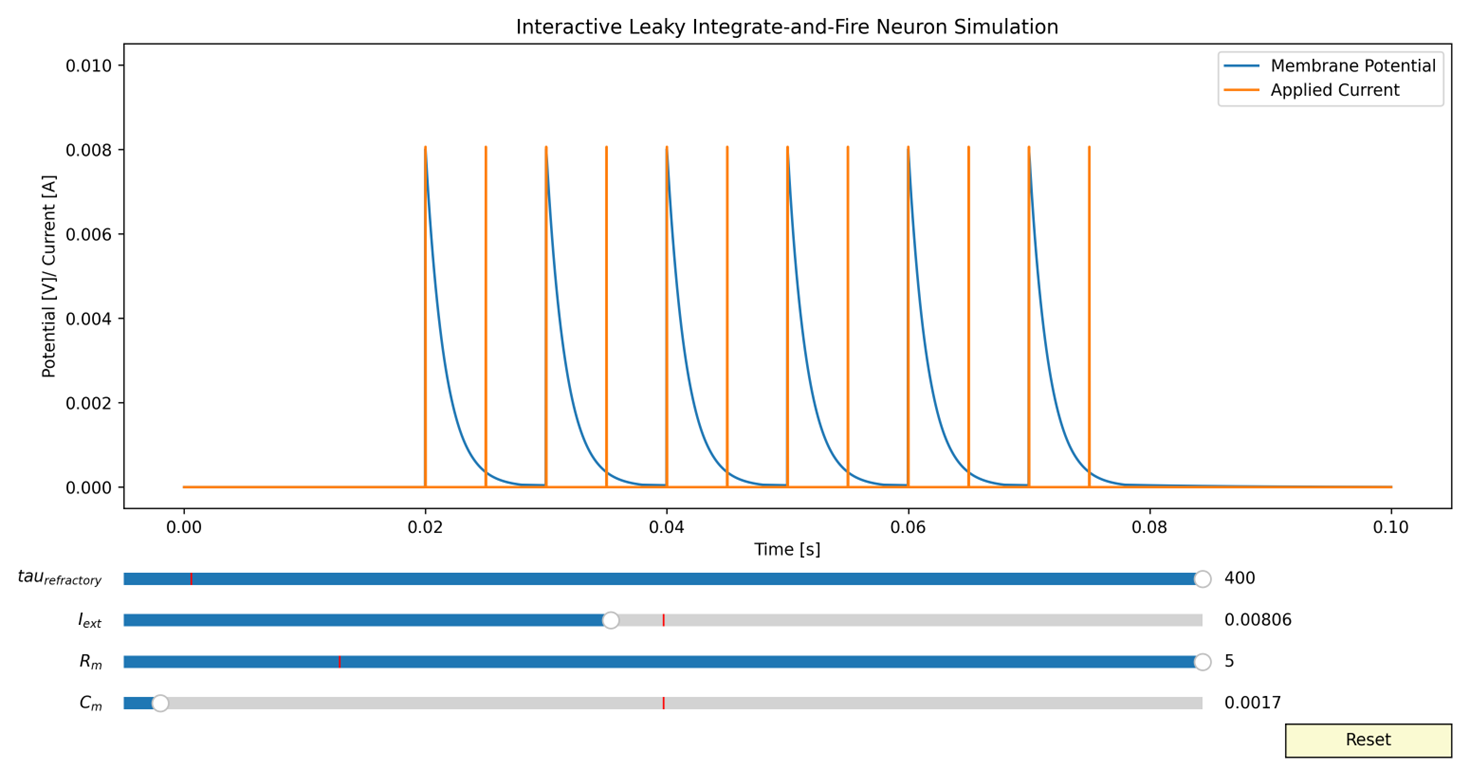
\includegraphics[width=0.8\textwidth]{methods/computational-models/graphs/LIF-spike-response-ref.png}
    \caption{LIF membrane voltage response to delta train input current}
    \label{fig:LIF-spike-ref}
\end{figure}

(*) for the above graph: \( I_0=V_{\text:thresh} \implies \) every input spike will cause the neuron to reach its action potential.

To demonstrate the sum of reactions of the given input:

\begin{figure}[H]
    \centering
    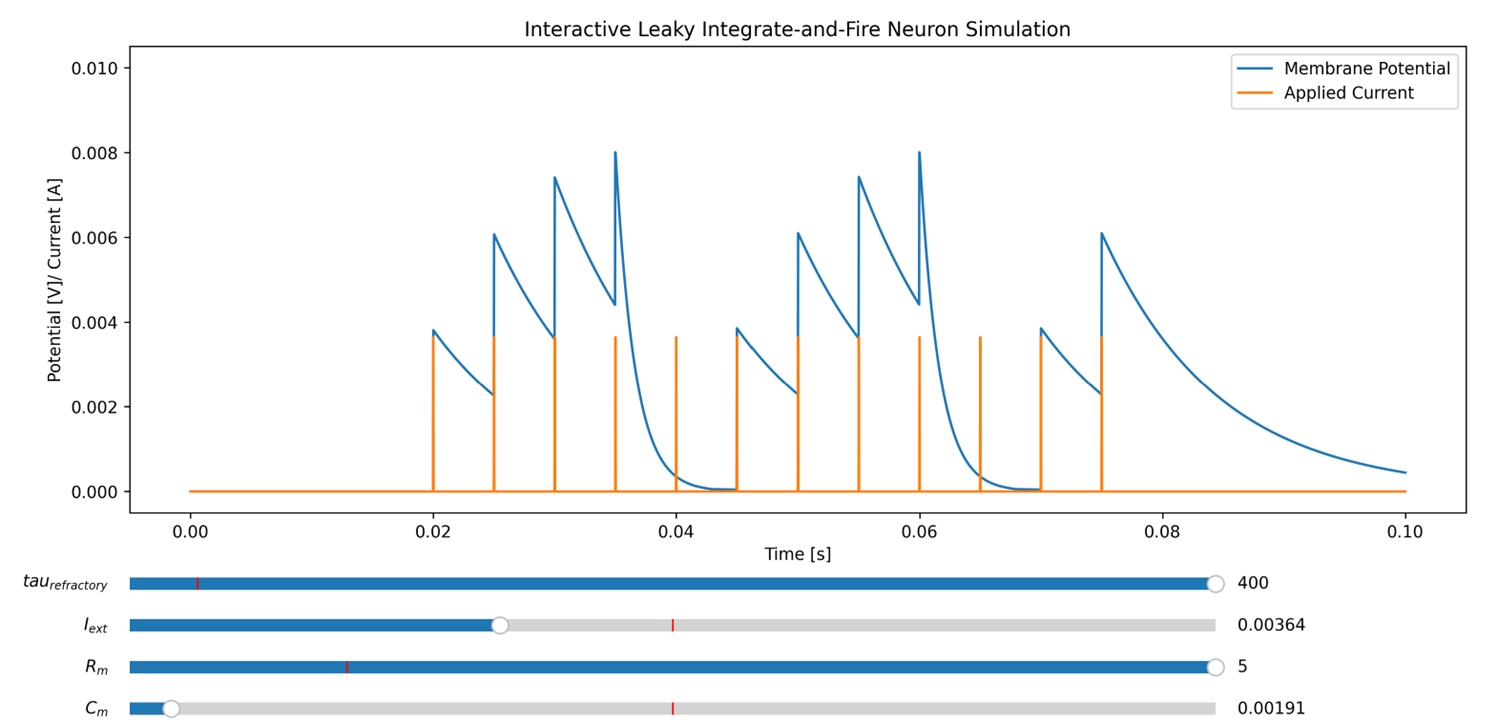
\includegraphics[width=0.8\textwidth]{methods/computational-models/graphs/LIF-high-freq-spike-response-ref.png}
    \caption{LIF membrane voltage response to high frequency delta train input current}
    \label{fig:LIF-high-freq-spike-ref}
\end{figure}

As we can see, when \(I_0 < V_{\text{thresh}}\), the voltage “spikes” for every \(I_0 \cdot \delta(t-t_i)\) till reaching the action potential and drops between input spikes. 

Let us take this a step further and find the firing frequency \(f(I_0, T)\) for a periodic delta train function:
\begin{equation}
I(t) = I_0 \cdot \sum_{n=0}^N \delta(t-n \cdot T)
\end{equation}
where \(T\) is the constant time period of the function and \(f = \frac{1}{T}\) is the frequency of the function.

For simplicity measures, we will assume: \(\tau_{\text{ref}} = 0\) and \(v_{\text{reset}} = 0\).
From the previous equation (7.1), we can conclude that the output for such an input will be:
\begin{equation}
v(t) = I_0 \cdot \sum_{n=0}^N H(t-n \cdot T) \cdot e^{-((t-n \cdot T)/\tau_m)}
\end{equation}

If \(v_{\text{th}} \leq I_0 \cdot \sum_{n=0}^{n_0} e^{-n \cdot T/\tau_m}\), then \(f(I_0, T) \geq \frac{1}{n_0} \cdot f\)

And if \(v_{\text{th}} \geq I_0 \cdot \sum_{n=0}^{n_0} e^{-n \cdot T/\tau_m}\), then \(f(I_0, T) \leq \frac{1}{n_0} \cdot f\)

Overall, we got:
\begin{equation}
f(I_0, T) = \frac{1}{n_0} \cdot f \quad \text{s.t.} \quad \sum_{n=0}^{n_0} e^{-n \cdot T/\tau_m} \leq v_{\text{th}} < I_0 \cdot \sum_{n=0}^{n_0+1} e^{-n \cdot T/\tau_m}
\end{equation}

The following graph will demonstrate the relation between \(f\), \(I_0\), and the firing frequency \(f(T, I_0)\):

\begin{figure}[H]
    \centering
    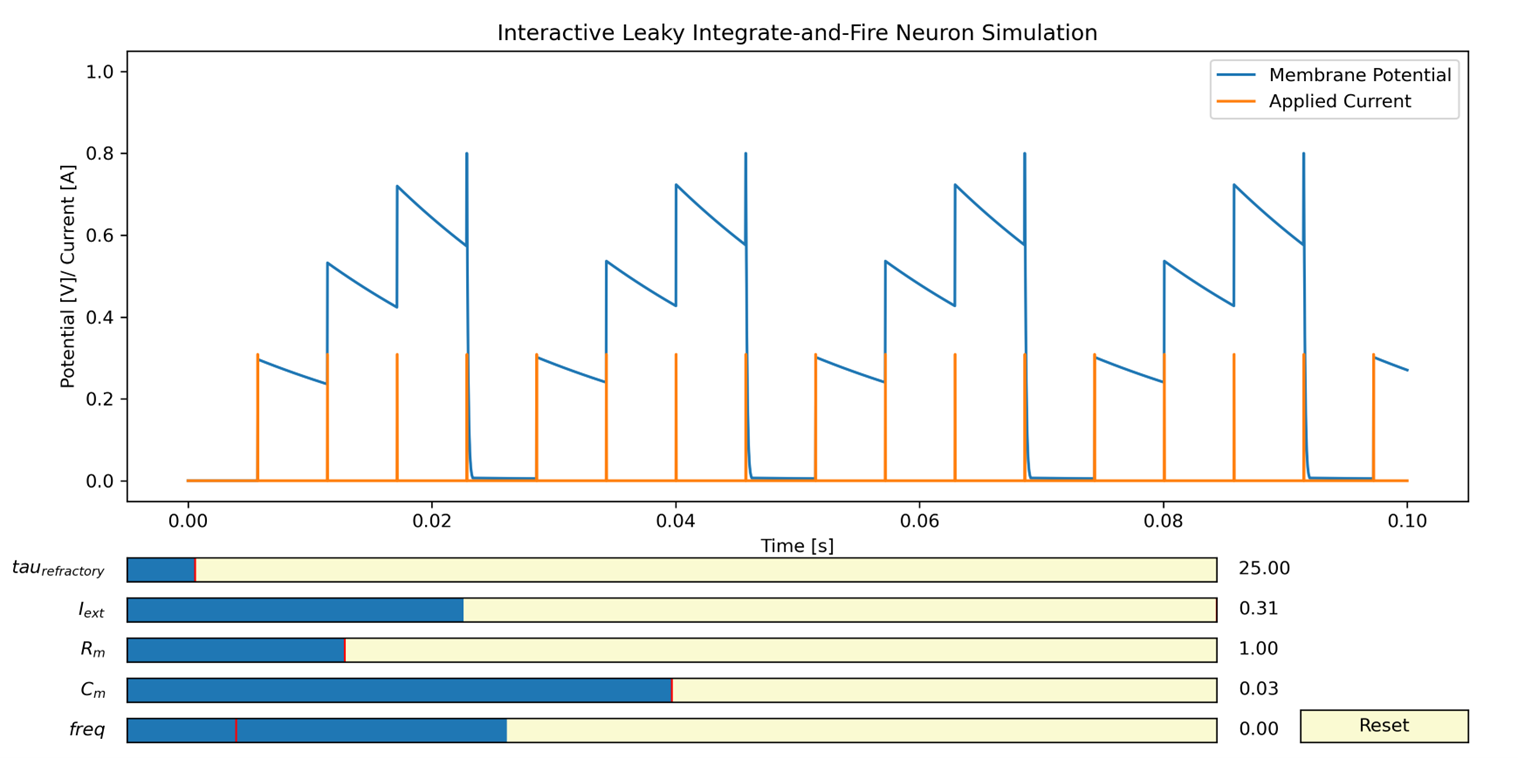
\includegraphics[width=0.8\textwidth]{methods/computational-models/graphs/LIF-high-freq-spike-response-ref-final.png}
    \caption{LIF membrane voltage response to high frequency delta spike trains with refractory period}
    \label{fig:LIF-high-freq-spike-ref-final}
\end{figure}


\subsection{General Solution}



\subsubsection{Double Exponent Model}

In this model, we have two variables: \\
\begin{enumerate}
    \item $v(t)$ represents the membrane potential of the neuron

    \item $I(t)$ represents the synaptic current.
\end{enumerate}

The term $\tau_m$ is the membrane time constant, and $\tau_s$ is the synaptic time constant. Both time constants determine how quickly the variables respond to changes in input.

The second-order low-pass filter model is represented by the following equations:

\begin{equation} \label{eq:def_eq_I}
    I(t) + \tau_s \frac{dI(t)}{dt} = I_{\text{in}}(t)
\end{equation}

\begin{equation} \label{eq:def_eq_V}
    v(t) + \tau_m \frac{dv(t)}{dt} = I(t)
\end{equation}

This model is motivated by the desire to capture more realistic neuronal dynamics. The first equation \ref{eq:def_eq_I} represents the dynamics of the input synaptic current, where $\tau_s$ controls how quickly the current responds to changes in input. The second equation \ref{eq:def_eq_V} represents the dynamics of the neuron's membrane potential, where $\tau_m$ determines the speed of the response to synaptic input.

\subsubsection*{Spike Response:}

To understand the spike response, let's consider the case of an impulse input current $I_{\text{in}}(t) = I_0 \delta(t)$ , where $I_0$ is the amplitude of the input current and $\delta(t)$ is the Dirac delta function.

In this case, the equations become:

\begin{equation} \label{eq:I_spike_res}
    I(t) + \tau_s \frac{dI(t)}{dt} = I_0 \delta(t)
\end{equation}

\begin{equation} \label{eq:V_spike_res}
    v(t) + \tau_m \frac{dv(t)}{dt} = I(t)
\end{equation}

Solving Equation \ref{eq:I_spike_res}: \\
We can solve Equation \ref{eq:I_spike_res} by taking the Laplace transform. The Laplace transform of the Dirac delta function as input is:

\begin{equation}
    I(s) + \tau_s s I(s) = I_0
\end{equation}

Solving for $I(s)$:

\begin{equation}
    I(s) = \frac{I_0}{1 + \tau_s s}
\end{equation}

Solving Equation \ref{eq:V_spike_res}: \\
Similarly, we take the Laplace transform of Equation \ref{eq:V_spike_res}:

\begin{equation}
    v(s) + \tau_m s v(s) = I(s)
\end{equation}

Substitute the expression for $I(s)$:

\begin{equation}
    v(s) + \tau_m s v(s) = \frac{I_0}{1 + \tau_s s}
\end{equation}

Solving for $v(s)$:

To obtain the time-domain solution from the Laplace domain, we use the method of partial fraction decomposition to rewrite the Laplace-domain expression in a form that allows us to take the inverse Laplace transform.

From Equation (10) in the previous response:

\begin{equation}
    v(s) = \frac{I_0}{(1 + \tau_s s)(1 + \tau_m s)}
\end{equation}

To decompose this expression into partial fractions, we need to find constants $A$ and $B$ such that:

\begin{equation}
    \frac{I_0}{(1 + \tau_s s)(1 + \tau_m s)} = \frac{A}{1 + \tau_s s} + \frac{B}{1 + \tau_m s}
\end{equation}

Now, we can find the values of $A$ and $B$ by equating the numerators:

\begin{equation}
    I_0 = A(1 + \tau_m s) + B(1 + \tau_s s)
\end{equation}

For simplicity, we can let $s = 0$ to find the value of $A$:

\begin{equation}
    I_0 = A
\end{equation}

Next, we can let $s = -\frac{1}{\tau_s}$ to find the value of $B$:

\begin{equation}
    I_0 = B\left(1 - \frac{\tau_s}{\tau_m}\right)
\end{equation}

Solving for $B$:

\begin{equation}
    B = \frac{I_0}{1 - \frac{\tau_s}{\tau_m}} = \frac{I_0}{\frac{\tau_m - \tau_s}{\tau_m}} = \frac{I_0 \tau_m}{\tau_m - \tau_s}
\end{equation}

Now that we have the values of $A$ and $B$, we can rewrite the Laplace-domain expression in terms of partial fractions:

\begin{equation}
    v(s) = \frac{I_0}{(1 + \tau_s s)(1 + \tau_m s)} = \frac{I_0}{\tau_m - \tau_s} \left(\frac{\tau_m}{1 + \tau_m s} - \frac{\tau_s}{1 + \tau_s s}\right)
\end{equation}

To take the inverse Laplace transform, we use standard Laplace transform pairs. The inverse Laplace transform of $\frac{\tau_m}{1 + \tau_m s}$ is $e^{-\frac{t}{\tau_m}}$, and the inverse Laplace transform of $\frac{\tau_s}{1 + \tau_s s}$ is $e^{-\frac{t}{\tau_s}}$. Thus, the time-domain solution for the membrane potential $v(t)$ is:

\begin{equation}
    v(t) = \frac{I_0}{\tau_m - \tau_s} \left(e^{-\frac{t}{\tau_m}} - e^{-\frac{t}{\tau_s}}\right)
\end{equation}

This is the double exponential spike response of the neuron's membrane potential to an impulse input current $I_{\text{in}}(t) = I_0 \delta(t)$. \\
The solution is characterized by two time constants: $\tau_m$ and $\tau_s$. The first term with $\tau_m$ dominates at short timescales, representing the fast response of the neuron, while the second term with $\tau_s$ governs the slower response at longer timescales.

We can normalize it into:

\begin{equation}
    v(t) = v_0 \cdot (e^{-t/\tau_m} - e^{-t/\tau_s})
\end{equation}

\begin{figure}[H]
    \centering
    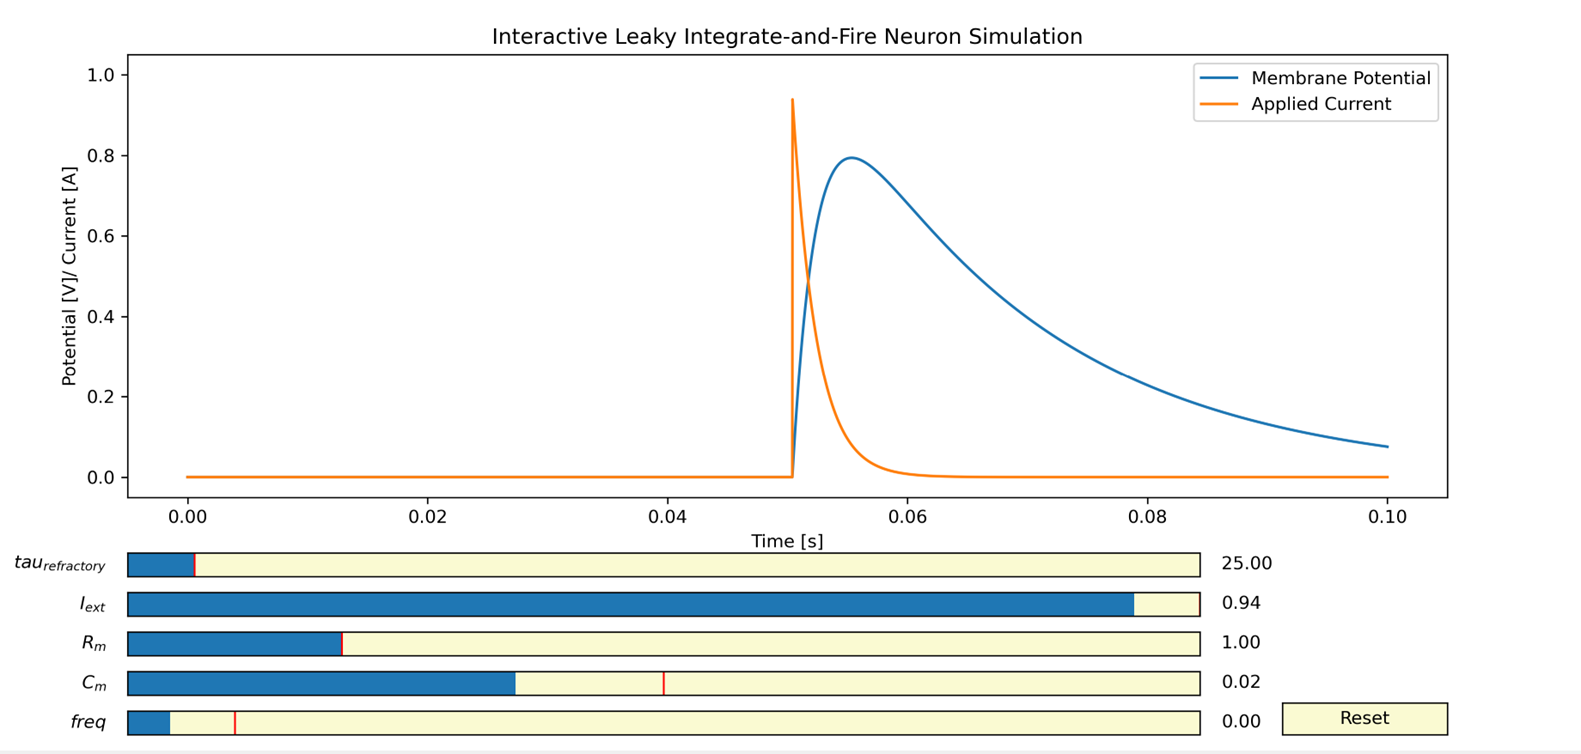
\includegraphics[width=0.6\textwidth]{scientific-background/computational-models/LIF/graphs/LIF-second-order.png}
    \caption{LIF 2-order membrane voltage response to spike}
    \label{fig:LIF-second-order}
\end{figure}

A useful definition will be:

\begin{equation}
    k(t) = v_0 \cdot (e^{-t/\tau_m} - e^{-t/\tau_s})
\end{equation}

So, the solution for:

\begin{equation}
    v(t) = \sum_{t^l} k(t - t^l)
\end{equation}

\begin{figure}[H]
    \centering
    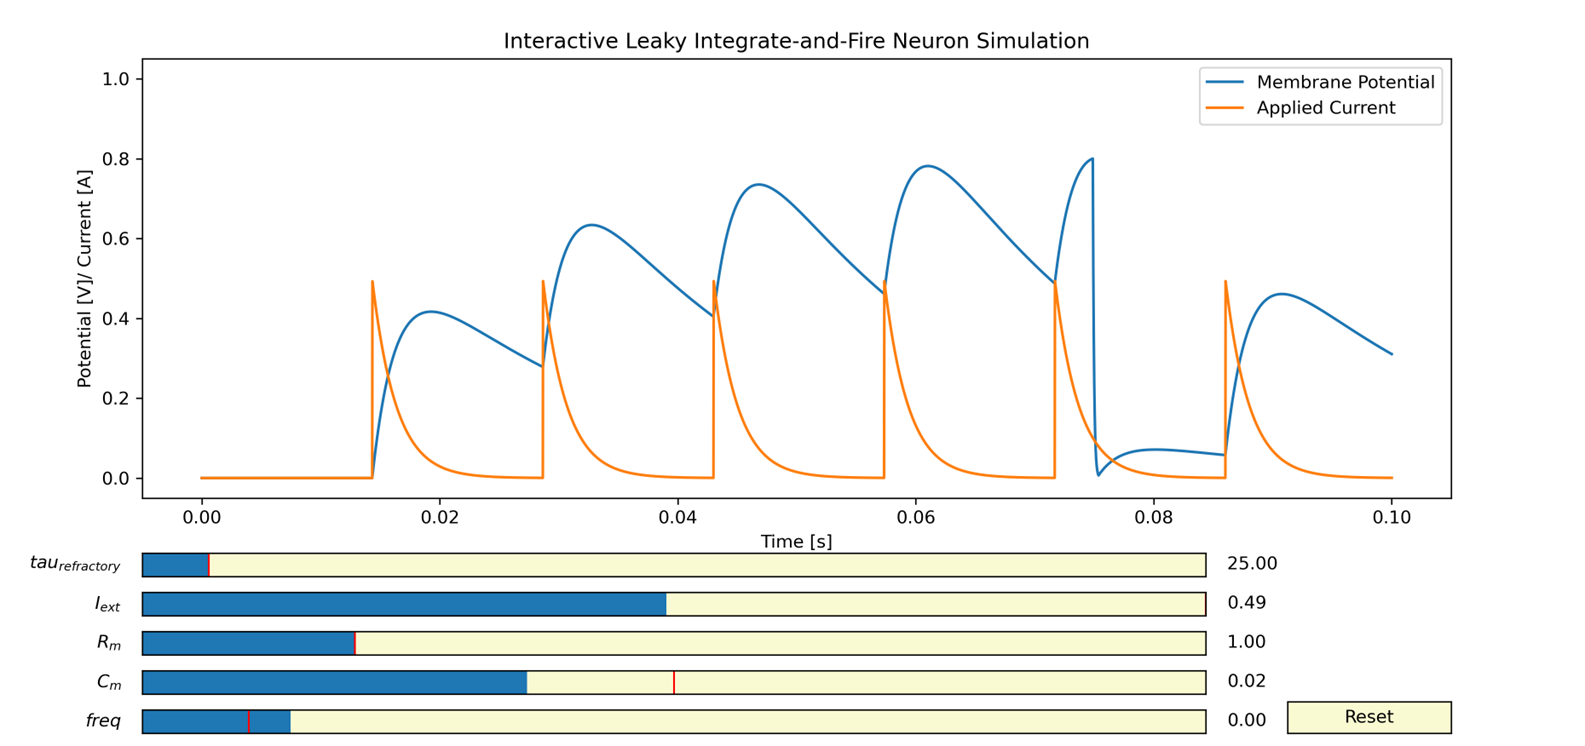
\includegraphics[width=0.6\textwidth]{scientific-background/computational-models/LIF/graphs/LIF-spike-response-second-order.png}
    \caption{LIF 2-order membrane voltage response to multiple spikes}
    \label{fig:LIF-second-order-spike-response}
\end{figure}

\chapter{Results}
\label{chap:results}


\section{Binary Classification}


\section{The Impact of Input Complexity on Tempotron Performance}

\subsection{Experimental Framework}

The primary objective of this investigation is to evaluate the performance trajectory of the Tempotron model in response to varying degrees of input complexity. The complexity measure, \( \alpha \), represents the ratio of distinct spike patterns \( P \) to the total number of input neurons \( N \):
\[ \alpha = \frac{P}{N} \]


\subsection{Input Data Synthesis}

Spike sequences were generated to ensure each neuron emits a solitary spike at random intervals, creating a myriad of unique patterns as governed by the \( \alpha \) ratio.

\subsection{Model Architecture}

The Tempotron model's design and operational mechanics are primarily defined in \ref{st:GD-simple-medel}


\subsection{Procedure}

For each selected \( \alpha \) value, multiple experimental trials were executed, each undergoing a preset number of learning iterations, processing data in specified batch sizes.



\subsection{Parameter Descriptions}

\begin{enumerate}
    \item \textbf{Duration \( T \): 500 ms} \\
    Represents the length of time for which the model will simulate the neural dynamics for each given input pattern.
    
    \item \textbf{Time step \( dt \): 1 ms} \\
    The sampling time at which we "measure" the experiment.
    
    \item \textbf{Resting potential \( V_0 \): 2.12} 
    
    \item \textbf{Firing threshold \( V_{th} \): 1} \\
    The potential level at which a neuron emits a spike. When the neuron's membrane potential exceeds \( V_{th} \), it "fires" or produces an output spike.
    
    \item \textbf{Time constant \( \tau \): 10 ms} \\
    Determines the rate at which a neuron's membrane potential decays back towards its resting potential after perturbation.
    
    \item \textbf{Output layer size: 1 neuron} \\
    Indicates the number of neurons in the model's final layer, which produces the final decision or classification.
    
    \item \textbf{Maximum iterations: 750} 

    \item \textbf{Batch size: 64} \\
    Dictates how many input patterns are processed simultaneously before updating the model's internal parameters. 

\end{enumerate}

\subsection{Results}

\begin{figure}[H]
    \centering
    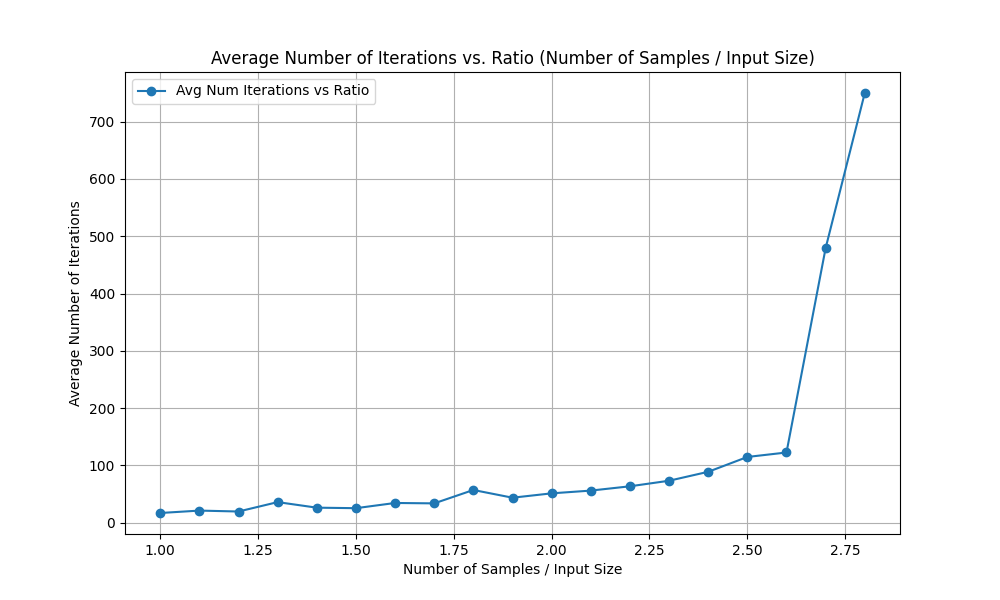
\includegraphics[width=0.8\linewidth]{results/graphs/alpha-validation.png}
    \caption{Number of training iterations until 100\% accuracy on the training data as a function of the ratio between the number of patterns and the input size}
    \label{fig:alpha-validation}
\end{figure}


\subsection{Observation}

The data collected from the experiment showcases the relationship between the ratio (\( \alpha \)) of different input patterns to neurons in the input layer and the average number of iterations required for the Tempotron to converge.

\textbf{Extreme Complexity Region (\( \alpha \geq\) 2.9)}: \\
Notably, at \( \alpha = 2.8 \), the average epochs reach the maximum value of 750, which was our defined limit. This may hint at a failure to converge, indicating that the Tempotron finds it virtually impossible to discern patterns at such high complexities using the given parameters.

Several factors might contribute to these observations:

\begin{itemize}
    \item The inherent design of the Tempotron, which relies on the temporal dynamics of spikes, may find it challenging to discriminate between overlapping or similar spike patterns as \( \alpha \) grows.
    
    \item The fixed parameters, such as the firing threshold \( V_{th} \) or the time constant \( \tau \), may not be optimal for handling higher complexity ratios. Adaptive mechanisms or parameter tuning might be necessary for such scenarios.
    
\end{itemize}

In conclusion, the Tempotron exhibits strong performance in classifying time-dependent, its capability goes beyond the recognized limit of \( \alpha = 2 \) for a single-layer perceptron \cite{gutig2006tempotron}. This fact is a strong foundation on which we rely our hipthesis that the Tempotron holds significant structural and ? benefits over the perceptron

In conclusion, the Tempotron demonstrates strong performance in classifying time-dependent patterns. Remarkably, its capacity surpasses the recognized threshold of \( \alpha = 2 \) associated with a single-layer perceptron \cite{gutig2006tempotron}. This observation forms a basis for our hypothesis that the Tempotron offers substantial structural and functional advantages over the perceptron.



\input{results/binary-classification/mnist/ch-beta-validation}

\input{results/binary-classification/mnist/ch-tau-validation}

\chapter{Conclusion}
\label{chap:conclusion}



\bibliographystyle{apalike}
\bibliography{thesis}

\end{document}